%%%%%%%%%%%%%%%%%%%%%%%%%%%%%%%%%%%%%%%%%
% Beamer Presentation
% LaTeX Template
% Version 1.0 (10/11/12)
%
% This template has been downloaded from:
% http://www.LaTeXTemplates.com
%
% License:
% CC BY-NC-SA 3.0 (http://creativecommons.org/licenses/by-nc-sa/3.0/)
%
%%%%%%%%%%%%%%%%%%%%%%%%%%%%%%%%%%%%%%%%%

%----------------------------------------------------------------------------------------
%	PACKAGES AND THEMES
%----------------------------------------------------------------------------------------

\documentclass{beamer}

\mode<presentation> {

% The Beamer class comes with a number of default slide themes
% which change the colors and layouts of slides. Below this is a list
% of all the themes, uncomment each in turn to see what they look like.

%\usetheme{default}
%\usetheme{AnnArbor}
%\usetheme{Antibes}
%\usetheme{Bergen}
%\usetheme{Berkeley}
%\usetheme{Berlin}
\usetheme{Boadilla}
%\usetheme{CambridgeUS}
%\usetheme{Copenhagen}
%\usetheme{Darmstadt}
%\usetheme{Dresden}
%\usetheme{Frankfurt}
%\usetheme{Goettingen}
%\usetheme{Hannover}
%\usetheme{Ilmenau}
%\usetheme{JuanLesPins}
%\usetheme{Luebeck}
%\usetheme{Madrid}
%\usetheme{Malmoe}
%\usetheme{Marburg}
%\usetheme{Montpellier}
%\usetheme{PaloAlto}
%\usetheme{Pittsburgh}
%\usetheme{Rochester}
%\usetheme{Singapore}
%\usetheme{Szeged}
%\usetheme{Warsaw}

% As well as themes, the Beamer class has a number of color themes
% for any slide theme. Uncomment each of these in turn to see how it
% changes the colors of your current slide theme.

%\usecolortheme{albatross}
%\usecolortheme{beaver}
%\usecolortheme{beetle}
%\usecolortheme{crane}
%\usecolortheme{dolphin}
%\usecolortheme{dove}
%\usecolortheme{fly}
%\usecolortheme{lily}
%\usecolortheme{orchid}
%\usecolortheme{rose}
%\usecolortheme{seagull}
%\usecolortheme{seahorse}
%\usecolortheme{whale}
\usecolortheme{wolverine}

%\setbeamertemplate{footline} % To remove the footer line in all slides uncomment this line
\setbeamertemplate{footline}[page number] % To replace the footer line in all slides with a simple slide count uncomment this line

\setbeamertemplate{navigation symbols}{} % To remove the navigation symbols from the bottom of all slides uncomment this line
}

\setbeamertemplate{bibliography item}{\insertbiblabel}


\usepackage{graphicx} % Allows including images
\usepackage{booktabs} % Allows the use of \toprule, \midrule and \bottomrule in tables
%\usepackage {tikz}
\usepackage{tkz-graph}
\usepackage{bibentry}


\usepackage[
backend=biber,
style=numeric,
sorting=ynt
]{biblatex}
 
\documentclass[xcolor=table]{beamer} 

\bibliography{bibfile}

\graphicspath{ {images/} }

\GraphInit[vstyle = Shade]
\tikzset{
  LabelStyle/.style = { rectangle, rounded corners, draw,
                        minimum width = 2em, fill = yellow!50,
                        text = red, font = \bfseries },
  VertexStyle/.append style = { inner sep=5pt,
                                font = \normalsize\bfseries},
  EdgeStyle/.append style = {->, bend left} }
\usetikzlibrary {positioning}
%\usepackage {xcolor}
\definecolor {processblue}{cmyk}{0.96,0,0,0}

% show sections only
\setcounter{tocdepth}{1}
% show subsections
%\setcounter{tocdepth}{2}
% show subsubsections
%\setcounter{tocdepth}{3}
\AtBeginSection[]
{
    \begin{frame}
        \frametitle{Table of Contents}
        \tableofcontents[currentsection]
    \end{frame}
}

%\AtBeginSubsection[]
%{
%    \begin{frame}
%        \frametitle{Table of Contents}
%        \tableofcontents[currentsection,currentsubsection]
%    \end{frame}
%}

%----------------------------------------------------------------------------------------
%	TITLE PAGE
%----------------------------------------------------------------------------------------

\title[Short title]{Thesis Pre-final presentation} % The short title appears at the bottom of every slide, the full title is only on the title page

\author{Azcarraga, Araya} % Your name
\institute[Department of Computer Science, University of the Philippine - Diliman] % Your institution as it will appear on the bottom of every slide, may be shorthand to save space
{
University of the Philippine - Diliman\\ % Your institution for the title page
\medskip
}
\date{\today} % Date, can be changed to a custom date

\begin{document}

\begin{frame}
\titlepage % Print the title page as the first slide
\end{frame}

\begin{frame}
\frametitle{Overview} % Table of contents slide, comment this block out to remove it
\tableofcontents % Throughout your presentation, if you choose to use \section{} and \subsection{} commands, these will automatically be printed on this slide as an overview of your presentation
\end{frame}

%----------------------------------------------------------------------------------------
%	PRESENTATION SLIDES
%----------------------------------------------------------------------------------------

%------------------------------------------------
\section{Introduction}

% to do sa intro
% list all jargon
% explain most jargon
% iklian bio part
% pahabain tech part esp p2p
% explain CDN

    %%%%%%%%%%%%%%%%%%% BIO SLIDES %%%%%%%%%%%%%%%%%%%%%%%%%%
    
    
    
    \subsection{Definition} %keep daw
    \begin{frame}{Human Karyotype}
        \centering
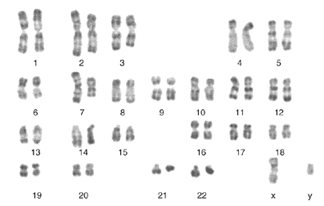
\includegraphics[scale=1]{karyotype.jpg}
    \end{frame}
    \begin{frame}{Definition of Genomics}
        According to the National Institute of Health \textit{Specifically for the Human Genome Project}
                \begin{block} {\textbf{Definition of Genomics}}
        Genomics is the study of all of a person's genes (the genome), including interactions of those genes with each other and with the person's environment. \cite{genomics-definition}
                \end{block}
    The genomics definition we will use is for \textbf{all} organisms
    \end{frame}
    
    
    \subsection{Introduction}
    \begin{frame}{Introduction}
        \begin{itemize}
            \item DNA comprises of the components A,T,G,C
            \begin{itemize}
                \item \textbf{A} - Adenine
                \item \textbf{T} - Thymine
                \item \textbf{G} - Guanine
                \item \textbf{C} - Cytosine
            \end{itemize}
            \item There needs to be a lot of these components to describe complex organisms
            \begin{itemize}
                \item The full human genome contains around $3.2 x 10^9$ base pairs \cite[p.~4]{introgenomics}
            \end{itemize}
        \end{itemize}
        \centering
        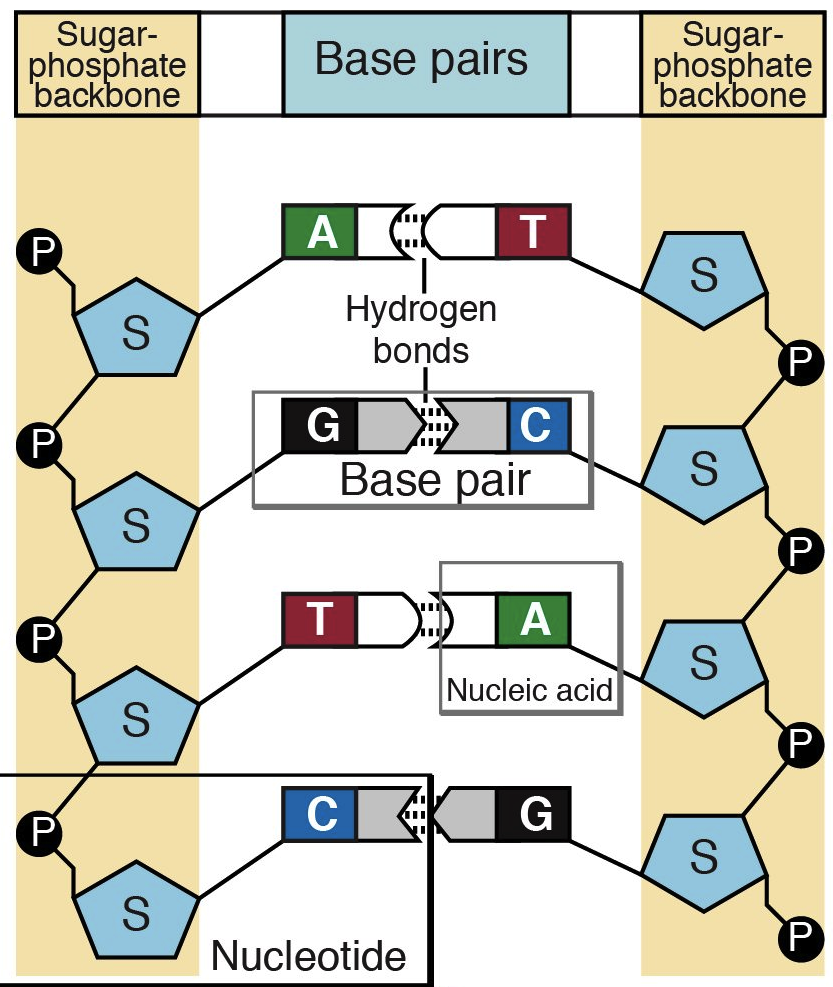
\includegraphics[scale=0.1]{gene-base-pair.png}
    \end{frame}
    
    \subsection{Genomics Data}
    \begin{frame}{Genomics Data}
            \textbf{Data Type}
    \begin{itemize}
        \item Store DNA sequences digitally
        \item A simple data file format is called FASTA format
            \begin{itemize}
                \item starts with $>$
                \item then can add keywords and attributes separated by $|$
            \end{itemize}
    \end{itemize}
    \begin{block}{Sample.FASTA}
    $>$AB000263 $|$acc=AB000263$|$descr=Homo sapiens mRNA for prepro cortistatin like peptide, complete cds.$|$len=70
ACAAGATGCCATTGTCCCCCGGCCTCCTGCTGCTGCTGCTCTCCGGGGCCACGGCCACCGCTGCCCTGCC

    \end{block}
    \end{frame}
    
    \subsection{Sequencing}
    \begin{frame}{Sequencing}
        \textbf{Sequencing}
    \begin{itemize}
        \item Sequencers are machines used to look at the DNA of a specimen (A,G,C,T)
        \begin{itemize}
            \item Sequencers look at the exact order of a single strand \cite{genomics-definition}. 
        \end{itemize}
        \item DNA is \textbf{replicated} and fragmented before processing
        \item Sequencers then reads (or sequences) them
        \item Output of the read fragments is contained in a .FASTA file
    \end{itemize}
            \centering
        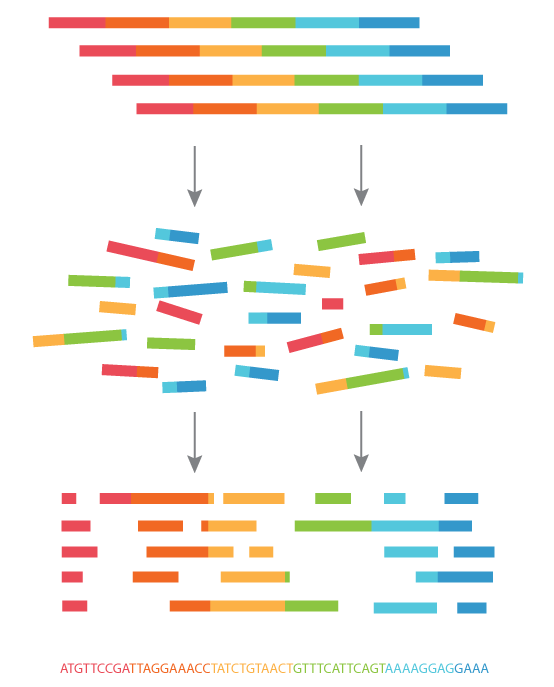
\includegraphics[scale=0.2]{sequencing.png}
    \end{frame}
    
    \begin{frame}{Next Generation Sequencing}
    (2003) The first human genome took ten years of work and $3,000,000,000$ \$ to finish.
    \begin{itemize}
        \item (2019) Currently the technology today in Japan can make 10,000 human genomes per day (Timewise: 36.5 million times faster) \cite[p.~19]{introgenomics}
    \end{itemize}
    \textbf{Next Generation Sequencers}
        \begin{itemize}
        \item Can read more faster, and cheaper
        \item More data
        \item Technology will get faster, there needs to be systems in preparation for that
    \end{itemize}
    \end{frame}
    %%%%%%%%%%%%%%%%%%% TECH SLIDES %%%%%%%%%%%%%%%%%%%%%%%%%%
    
    \subsection{Data Storage}
    \begin{frame}{Data Storage}
        A \textbf{database} (\textbf{DBMS}, Database Management System) is defined by 
        \begin{block} {\textbf{Definition}}

        DBMS contains information about a particular enterprise
        \begin{itemize}
            \item Collection of interrelated data
            \item Set of programs to access the data 
            \item An environment that is both convenient and efficient to use
        \end{itemize}
        \cite{Silberschatz2010}
        \end{block}
    \end{frame}
    
    \subsection{Database Principles}
    \begin{frame}{Database Principles}
        \begin{itemize}
            \item \textbf{Principles} to remember when creating a database (CAP). Idea is that only 2 of the three can be focused on. \cite[Ch.~19]{Silberschatz2010}
            \begin{itemize}
                \item \textbf{Consistency}
                \begin{itemize}
                    \item Update one part, will all other (replicated) parts be updated quickly as well
                    \item Data is accurate and copied faithfully
                \end{itemize}
                \item \textbf{Accessibility}
                \begin{itemize}
                    \item How easy it is to access data
                    \item API protocols
                \end{itemize}
                \item  \textbf{Partition Tolerance}
                \begin{itemize}
                    \item If one portion breaks, the other portions are still usable
                    \centering 
                    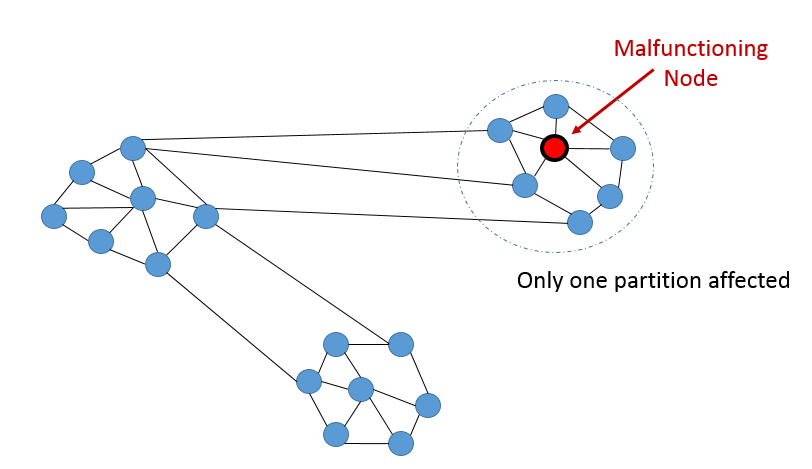
\includegraphics[scale=0.2]{partition_tolerance.png}
                    \end{itemize} 
             \end{itemize}
        \end{itemize}
    \end{frame}
    
    \subsection{Special Database}
    \begin{frame}{Special Databases}
        \textbf{Large Data}
        \begin{itemize}
            \item \textbf{Distributed Database}
            \begin{itemize}
                \item A distributed database system consists of loosely coupled sites that share no physical component             
                \item Database systems that run on each site are independent of each other
                \item Transactions may access data at one or more sites
                \cite[Ch.~19]{Silberschatz2010}
                \item Beneficial for large data with a certain speed requirement
            \end{itemize}
        \end{itemize}
    \end{frame}

    \begin{frame}{Special Databases}
        \textbf{Genomics Data}
        \texttt{needs a different set of features to easily conduct processes (alignment, assembly, comparison).}
        \begin{itemize}
            \item Need a special database to store all of these data
            \item Designed for more efficient and optimal use
            \item Has special needs for the users of genomic data
            \item Discuss in the RRL the different ways researchers approached this
        \end{itemize}
    \end{frame}
    
        \begin{frame}{Network Layers}
         \textbf{Networks Layers} how computers pass data to each other
        \begin{itemize}
            \item \begin{itemize}
            \item Level 1: Medium used to send signals (physical, electrical signals of 0 and 1), through wire or by air
            \item Level 2: Introduction of packets: Wifi, Ethernet, connecting together different . Goal of sending a group of signals.
            \item Level 3: Introduction of networks: IP Address to uniquely identify entities. 
            \item Level 4: Management of error free data transmission: Sending a group of messages via TCP, UDP, FTP
            \item \textbf{Level 5}: Abstraction of Level 4: Function calls programmers will use to do level 4 processes.
            \end{itemize}
        \end{itemize}
    \end{frame}
    
    \subsection{Application Architecture}
    \begin{frame}{Application Architecture}
        \begin{itemize}
            \item The \textbf{application architecture} is how a networked app is structured across the various end systems (i.e. computers, servers, etc.) \cite{kurose}
            \item Falls into either client-server, peer-to-peer, or hybrid architecture
        \end{itemize}
    \end{frame}
        \subsubsection{Client-Server}
        \begin{frame}{Client-Server}
            \begin{itemize}
                \item A \textbf{client-server} architecture relies on a Web server that is always available and has a fixed IP address\\
                \item A single server connects to many clients
            \end{itemize}
            \centering
            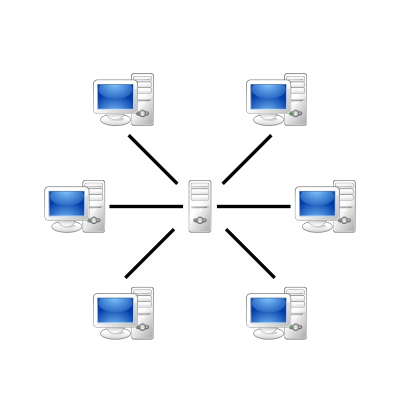
\includegraphics[scale=0.5]{Server-based-network.png}
        \end{frame}
        \subsubsection{Peer-to-Peer \& Hybrid}
        \begin{frame}{Peer-to-Peer \& Hybrid}
            \begin{itemize}
                \item A \textbf{peer-to-peer (P2P)} architecture has minimal to no reliance on always-on, dedicated servers
                \item Peers are desktops/laptops that communicate to each other without passing through a dedicated server
                \item A \textbf{hybrid} architecture combines elements of P2P and client-server architectures, attempting to utilize advantages of both
            \end{itemize}
            \centering
            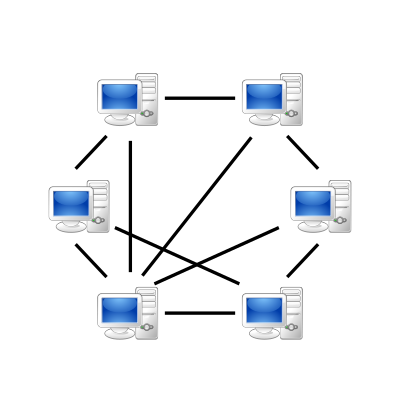
\includegraphics[scale=0.5]{P2P-network.png}
        \end{frame}
        \begin{frame}{BitTorrent terminology}
            \begin{itemize} % siguro breeze through what these mean 
                \item \textbf{Peers} are users that connect to the BitTorrent network.
                \item \textbf{Torrent files} contain metadata about files \& folders, trackers, and hash values.
                \item \textbf{Trackers} are servers that keep track of peers and availability of files
                \item \textbf{Seeds} are peers which have downloaded the entire file and are making it available
            \end{itemize}
        \end{frame}

\section{Review of Related Literature}
    \subsection{BioTorrents}
    \begin{frame}{BioTorrents}
        % outline
        \begin{itemize}
        \item System for legally sharing scientific data that works on top of the BitTorrent protocol. It is much like a public tracker.
        \item The main website hosts .torrent and metadata files
        \item Info about each dataset includes categories, license, filenames, etc. that helps users in searching for relevant datasets
        \item Torrent file has list of trackers, servers that "know" which peers are serving which files.
        \item Torrent client downloads from multiple peers simultaneously.
        \item To upload a torrent, the client makes a .torrent file using the torrenting software, then uploads it to the main website along with metadata. The client must have their computer continuously turned on to keep the file available as a peer. \cite{biotorrents}
        \end{itemize}
    \end{frame}
    
    \begin{frame}{BioTorrents}
        \begin{itemize}
            \item As with all public trackers, BioTorrents requires "good souls" that will keep many torrents available as often as possible.
            \item The datasets must be moderated to prevent abuse.
            \item The BioTorrents website is no longer up.
        \end{itemize}
    \end{frame}
 
    
    \subsection{PeerDB}
    \begin{frame}{PeerDB}
        \begin{itemize}
            \item Proposed P2P system for sharing general data
            \item Each node is equipped with a database
            \item Queries are passed around neighbors, with a maximum number of hops
            \item Caches information about other peers to speed up queries
            \item Large number of nodes & relatively small number of lookup servers
            \cite{peerdb}
        \end{itemize}
    \end{frame}

    
    \subsection{SeqTorr}
    \begin{frame}{SeqTorr}
    \textbf{SeqTorr} \cite{seqtorr}
    \begin{itemize}
        \item Utilizes distributed database
        \item Master node
        \begin{itemize}
            \item containing metadata of all the sequences
            \item where user authentication is handled
        \end{itemize}
        \item Data node
        \begin{itemize}
            \item contain a portion of all the sequences
            \item needs to replicate a sequence \texttt{r} times before a sequence is considered available
            \item proximity of data nodes can increase download speed but isn't true P2P
        \end{itemize}
        \item Defined API Implementation
        \begin{itemize}
            \item POST
            \item GET
            \item PUT
            \item DELETE
        \end{itemize}

    \end{itemize}
    \end{frame}
    
    
    \begin{frame}{SeqTorr}
        Problems:
        \begin{itemize}
            \item program not currently available
            \begin{itemize}
                \item cannot measure any statistics on this
            \end{itemize}
            \item not Peer2Peer
        \end{itemize}
    \end{frame}
    
    \begin{frame}{Table}
   \begin{table}[]
\begin{tabular}{|l|l|l|l|l|}
\hline
System      & CS/P2P/H & Available? & DL/UL speed & Type of Data \\ \hline
BioTorrents & P2P           & No         & Depends                    & Bio-related  \\ \hline
SeqTorr     & H             & No         & Fast (PH server)           & FASTA        \\ \hline
PeerDB      & P2P           & No         & Depends                    & General      \\ \hline
NCBI        & CS            & Yes        & Slow (US server)           & Bio-related  \\ \hline
\end{tabular}
\end{table} 
    \end{frame}

% NCBI Biosystems
% pros
% cons

% BitTorrious
% pros
% \cite{bittorious}
% cons

\section{Problem}
\begin{frame}{Problem}
The different gaps or problems found with other implementations

\begin{itemize}
    \item Genome researchers download entire database of genomic data
    \item Genome researchers only need a portion of the database, but end up downloading all
    \item Client-Server approach can face bottlenecks (server speed)
    \item Code has no documentation, thus harder to maintain
%% add more

\end{itemize}
\end{frame}

\section{Objectives}
\begin{frame}{Objectives}
Based on the problems we found earlier, we propose the following objectives
    \begin{itemize}
        \item Create information system that speeds up the download and upload of genomic data by at least 3x compared to existing systems
        \item The system should have the main API's
        \begin{itemize}
            \item POST genome data
            \item GET genome data (implement hybrid P2P)
            \item PUT genome metadata (optional: PUT data)
            \item DELETE genome data
        \end{itemize}
        \item Write documentation for the system
    \end{itemize}
\end{frame}

\section{Scope}
\begin{frame}{Scope}
The current scope and coverage of the project is only
\begin{itemize}
    \item Security and Authentication is not part of the scope
    \item Use only FASTA file format 
    \begin{itemize}
        \item DNA nucleotides only
    \end{itemize}
    \item UI will be purely for functional purposes (very basic design)
\end{itemize}
\end{frame}

\section{Theoretical Framework}

\begin{frame}{Theoretical Framework: System Description}
    \begin{itemize}
        \item A \textbf{master node} stores metadata of all sequences, may or may not contain sequence files
        \item \textbf{Data nodes} stores sequence files & metadata of all sequence files in its filesystem
        \item Both master node & data nodes have user interface that allow users to upload, search, and download sequence files
    \end{itemize}
\end{frame}
% DRAW.IO FILE: https://drive.google.com/file/d/1Nbp0Kmgcr2BZ13LBT3SGLMBoA6JA_Eth/view
\begin{frame}{Theoretical Framework: Schematics}
\textbf{App network diagram} \\ \medskip
\centering
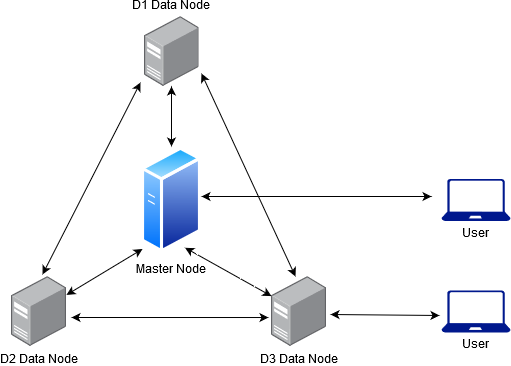
\includegraphics[scale=0.5]{thesis1.png}
\end{frame}

\begin{frame}{Theoretical Framework: Schematics}
\textbf{POST: Uploading a sequence to the master node} \\ \medskip
\centering
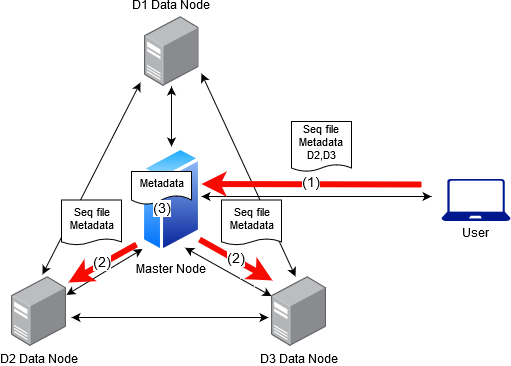
\includegraphics[scale=0.5]{thesis3.png}
\end{frame}

\begin{frame}{Theoretical Framework: Schematics}
\textbf{POST: Uploading a sequence to a data node} \\ \medskip
\centering
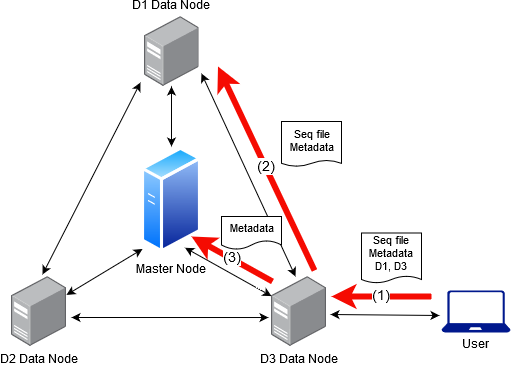
\includegraphics[scale=0.5]{thesis2.png}
\end{frame}

\begin{frame}{Theoretical Framework: Schematics}
\textbf{GET: Downloading a sequence} \\ \medskip
\centering
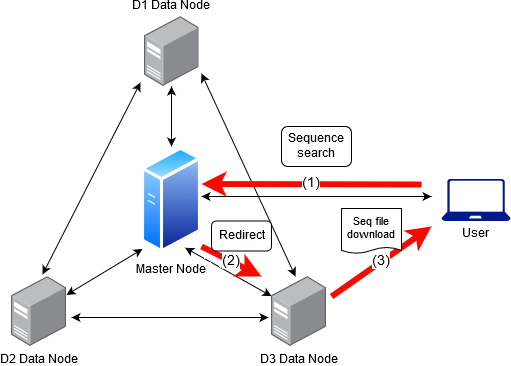
\includegraphics[scale=0.5]{thesis4.png}
\end{frame}

\section{Proposed Methodology}
\begin{frame}{Proposed Methodology}
\begin{enumerate}
    \item Creating the system
    \begin{enumerate}
        \item Make prototype for UI
        \item Code data node
        \item Deploy \& test functionality of data node/s
        \item Code master node
        \item Deploy \& test functionality of master node/s
        \item Test interoperability of nodes
    \end{enumerate}
    \item Benchmarking
    \begin{enumerate}
        \item Create test for testing original speed
        \item Test original download speeds
        \item Create test for testing new speed
        \item Test new speeds
    \end{enumerate}
        \item Documentation
    \begin{enumerate}
        \item PDF & Github Style
        \item How to use (all users)
        \item How to set up
        \item How to maintain & add features
        \item How to test?
    \end{enumerate}
\end{enumerate}
\end{frame}

\subsection{Proposed Methodology Timeline}
\begin{frame}{Proposed Methodology: Timeline 1}
    \begin{itemize}
        \item Mid January: Start
        \item Mid April: End
    \end{itemize}
    \begin{enumerate}
        \item End January Deliverable: 
        \begin{itemize}
            \item Wireframe Mockup
            \item Pseudocode / Flowchart of Entire System (to be reviewed by the adviser)
            \item Finalized feature list
            \item Documentation Version 1 (Cid)
        \end{itemize}
        \item End of February Deliverable:
            \begin{itemize}
                \item Benchmarking specifications finalization \& Set up
                \item Start of bench marking of existing tech
                \item Start Coding
                \item Documentation Version 2 (Cid)
            \end{itemize}
    \end{enumerate}            
            \end{frame}

    \begin{frame}{Proposed Methodology: Timeline 2}
        \begin{enumerate}  
        \item Mid March Deliverable:
            \begin{itemize}
                \item Finish Coding version 1 of system
                \item Implement basic UI
                \item Finish bench marking existing 
                \item Start Alpha Testing (us and other undergrad thesis students)
                \item Documentation Version 3 (Cid)
            \end{itemize}
        \item End of March Deliverable:
            \begin{itemize}
                \item Revise version 1 to version 2 of system based on Alpha Test
                \item Revise basic UI
                \item Testing of system for feature 
                \item Start Beta Testing (public, DCS \& PGC community)
                \item Documentation Version 4 (Cid)
            \end{itemize}
        \item Mid April Deliverable
            \begin{itemize}
                \item Revise version 2 to version 3 of system based on Beta test
                \item Documentation Version 5 (Cid)
            \end{itemize}
    \end{enumerate}
\end{frame}

\begin{frame}
\Huge{\centerline{The End}}
\small{\centerline{Thank you for coming}}
\end{frame}

\begin{frame}
\Huge{\centerline{Discussion points}}
\small{

\begin{itemize}
    \item What principles of database design will be focused here?
        \begin{itemize}
            \item Consistency
            \item Availability
            \item Partition Tolerance
        \end{itemize}
    \item Focus of the thesis?
    \begin{itemize}
        \item Not be focused on peer to peer? But peer to peer principles that solves the problems?
        \item Focused on making the data easier for users to get?
    \end{itemize}
    \item How will bench marking and testing be done?
    \begin{itemize}
        \item Download entire NCBI database?
        \item Download a portion?
        \item Download a specific genome (chicken / rice)?
    \end{itemize}
\end{itemize}

}
\end{frame}

\section{Bibliography}

\begin{frame}[allowframebreaks]
\printbibliography[heading=none]
\end{frame}


\end{document}

